% 等离子体基础第一次作业

\section{Saha ionization equation}
Saha 电离方程给出了温度、压强与热平衡下的电离了的气体电离度之间的关系。

在足够的温度和压力下
原子的热碰撞会电离一些原子,
形成一些电离了的气体。

% % 等离子体基础第一章

\section{等离子体基础第一章}
\subsection{德拜屏蔽}
\subsubsection{Debye 半径}
设电子(\(n_e\))与离子(\(n_i\))分别处于热平衡
\begin{equation}
  \laplacian \phi = - \frac{\rho}{\epsilon_0} = - \frac{1}{\epsilon_0} (  n_i Z_i e - n_e e )
\end{equation}
\begin{figure}[htpb]
  \centering
  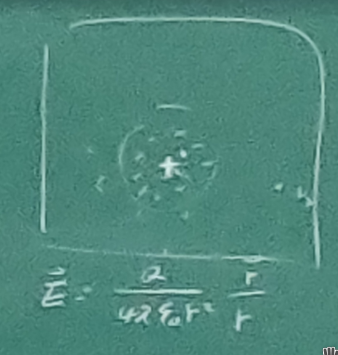
\includegraphics[width=0.3\linewidth]{figures/2022-09-09T221136+0800.png}
  \caption{法拉第笼的静电屏蔽}%
\end{figure}
设粒子数密度服从玻耳兹曼分布
\begin{gather}
  n_i = n_{i0} \exp(\frac{- Z_i e \phi}{T_i}) \\
  n_e = n_{e0} \exp(\frac{e \phi}{T_e})
\end{gather}
此处,\(e\phi \ll T_e, T_i\) and
\begin{align*}
  & n_{i 0 } = n_i (\phi = 0 ) \\
  & n_{e 0} = n_e (\phi = 0 )
\end{align*}
作泰勒展开\sn{\(1 + x + \frac{x^2}{2!}\)}
\begin{align*}
  & n_i \sim n_{i 0} \left(1 - \frac{Z_i e \phi}{T_i}\right) \\
  & n_e \sim n_{e 0} \left(1 + \frac{ e \phi}{T_e}\right)
\end{align*}
由于无穷远处等离子体呈准中性\(n_{e 0} e = n_{i 0} Z_i e\)
\begin{equation}
  \begin{aligned}
    \laplacian \phi &= \frac{1}{\epsilon_0} \left[
\left(1 + \frac{ e \phi}{T_e}\right)
- \left(1 - \frac{Z_i e \phi}{T_i}\right)\right] \\
                    &=
\frac{1}{\epsilon_0}\left(
\frac{ e \phi}{T_e} +
\frac{Z_i e \phi}{T_i}
\right)\phi
  \end{aligned}
\end{equation}
由于球对称性
\begin{equation}
  \frac{1}{r^2} \dv{r}(r^2 \dv{\phi}{r}) = \frac{1}{\lambda_d^2}\phi
  \label{eq:Debye_1}
\end{equation}
\begin{definition}[德拜半径]
  \begin{equation}
  \lambda_d = \left( \frac{n_{e0} e^2}{\epsilon_0 T_e}  + \frac{n_{i0}  (Z_i e)^2}{\epsilon_0 T_i}\right)^{- 1 / 2}
  \end{equation}
\end{definition}

\begin{remark}
  \begin{itemize}
    \item \(T_e  \gg  T_i\),德拜半径主要取决于电子项
    \item \(T_e  <<  T_i\),德拜半径主要取决于离子项
    \item \(T_e  \sim  T_i\)
  \end{itemize}
\end{remark}

\subsubsection{Debye 势}
设\(u = r \phi\), \cref{eq:Debye_1} 变为
\begin{equation}
 \dv[2]{u}{r}  - \frac{u}{\lambda_d^2} = 0
\end{equation}
解得
\begin{equation}
u = 
A \exp( - \frac{r}{\lambda_d} )
+B \exp( + \frac{r}{\lambda_d} )
\end{equation}
\begin{equation}
\phi = \frac{u}{r} =
\frac{A}{r} \exp( - \frac{r}{\lambda_d} )
+\frac{B}{r} \exp( + \frac{r}{\lambda_d} )
\end{equation}
根据边界条件
\begin{align}
  & \phi(r \to \infty) = 0 \implies B=0 \\
  & \phi(r \to 0) = \frac{q}{4 \pi \epsilon_0 r} \implies A = \frac{q}{4\pi \epsilon_0}
\end{align}
解得:
\begin{definition}[Debye-Huckel 势 或 YuKawa 势]
\begin{equation}
 \phi = \frac{q}{4 \pi \epsilon_0}  \frac{1}{r} \exp(- \frac{r}{\lambda_d})
\end{equation} 
\end{definition}
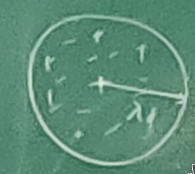
\includegraphics[width=0.3\textwidth]{figures/2022-09-09T230435+0800.png}

\subsubsection{德拜半径的物理意义}
\begin{itemize}
  \item 静电作用的屏蔽半径
\begin{itemize}
  \item \(L>\lambda_d\)静电势可以忽略
  \item \(L<\lambda_d\)静电势不可以忽略
\end{itemize}
\item 局域电荷分布的空间尺度
 \begin{itemize}
  \item \(L>\lambda_d\) 德拜球内电荷分离
  \item \(L<\lambda_d\) 德拜球外准中性
\end{itemize} 
\end{itemize}
所以,带电离子系统特征长度\(L \gg  \lambda_d\) 是等离子体的一个判据
\begin{gather*}
  \lambda_d \gg  d \\
  N = n \lambda_d^3 \gg  1  \\
  g = \frac{1}{n \lambda_d^3} \ll  1
\end{gather*}
特征长度
\begin{equation}
  \lambda_L : d : \lambda_d : \lambda_{\text{库伦}} = d : 1 : \frac{1}{2\sqrt{\pi \alpha}} : \frac{1}{\pi \alpha^2}
\end{equation}
对于高温低密度等体 \(\alpha \ll  1, \lambda_L \ll d \ll  \lambda_d \ll  \lambda_{\text{库近}}\)

\subsection{等离子体频率}
假设等离子体某一区域\(L > \lambda_d\)出现电子过剩,
多余电子产生电场
\(\implies\)
电场驱使电子向外运动
\(\implies\)
电中性
\(\implies\)
电子惯性,向外运动
\(\implies\)
反向电场
\(\implies\)
电子向内运动。
即等离子体振荡。

假设离子不动,电子移动\(x\)
于是电荷面密度为
\begin{equation}
\sigma = n_e e x
\end{equation}
电场为
\begin{equation}
  E = \frac{\sigma}{\epsilon_0}
\end{equation}
则运动方程
\begin{equation}
  m_e \dv[2]{x}{t} = - e E = - \frac{n_e e^2}{\epsilon_0} x
\end{equation}
\begin{definition}[等离子体电子振荡频率]
  \begin{equation}
  \omega_{pe} = \left( \frac{n_e e^2}{\epsilon_0 m_e} \right)^{1 / 2}
  \end{equation}
\end{definition}
\begin{definition}[等离子体离子振荡频率]
  \begin{equation}
  \omega_{pi} = \left( \frac{n_i e^2}{\epsilon_0 m_i} \right)^{1 / 2}
  \end{equation}
\end{definition}
\begin{equation*}
  \begin{aligned}
    \omega_{pe} \gg 
    \omega_{pi} \\
    \frac{\omega_{pe}}{\omega_{pi}} = \left( \frac{m_i}{m_e} \right)^{\frac{1}{2}}
  \end{aligned}
\end{equation*}
若电子离子运动,则以约化质量
\begin{equation}
  m = \frac{m_e m_i}{m_e + m_i}
\end{equation}
代替。
则
\begin{definition}[等离子体频率]
  \begin{equation}
  \omega_p^2 =  
  \omega_{pi}^2  +
  \omega_{pe}^2 
  \approx 
  \omega_{pe}^2 
  \end{equation}
\end{definition}

\subsubsection{振荡频率的物理意义} 
\begin{equation}
  x(t) = \underbrace{a}_{\text{振幅}} \cos(\omega_{pe} + \phi_0)
\end{equation}
振荡能量\(\frac{1}{2} m_e ( a \omega_{pe}^2 )\) 来源于热能
\begin{equation}
  \frac{1}{2} m_e (a \omega_{pe})^2 = \frac{1}{2} T_e = \frac{1}{2} m_e v_{th}^2
\end{equation}
\begin{equation}
  a = ( \frac{T_e}{m_e}^{1 / 2} \frac{1}{\omega_{pe}} ) = \frac{ V_{th} }{ \omega_{pe} } = \lambda_d
\end{equation}
\begin{remark}
  振幅为德拜长度,由于德拜长度为电荷分离的空间尺度。
\end{remark}




%%% vim: set ts=2 sts=2 sw=2 isk+=\: et cc=+1 formatoptions+=mM:


\section{等离子体基础第二章}

\subsection{带电离子在匀强恒定电磁场中的运动}
\subsubsection{}
令\(\va{\omega}_c = \frac{q \vb{B}}{m} \)有
\begin{equation}
  \dv{\vb{v}}{t} = - \va{\omega}_c \cross \vb{v}
\end{equation}

可知,
\begin{itemize}
  \item \(q=-e\),角速度与\(\vb{B}\)的方向相同
  \item \(q=e\),角速度与\(\vb{B}\)的方向相反
\end{itemize}
粒子体现抗磁效应。

回旋频率:
\begin{equation}
  \omega_c = \abs{\frac{qB}{m}}
\end{equation}
\(\omega_c\)为等离子体的几个基本时间尺度之一。
\(\omega_{ci} \ll  \omega_{ce}\),因为电子质量比较小,回旋更"快"。




%%% vim: set ts=2 sts=2 sw=2 isk+=\: et cc=+1 formatoptions+=mM:
